\documentclass[conference]{IEEEtran}
\IEEEoverridecommandlockouts
\usepackage[T1]{fontenc}
\usepackage{graphicx}
\usepackage{multicol}
\usepackage{url}
\usepackage{algpseudocode}
\usepackage{tikz}
\usetikzlibrary{arrows.meta}
\usepackage[hidelinks]{hyperref}
% Shared visual language for the implementation-derived state diagrams.
\definecolor{stateBlue}{HTML}{355D8A}
\definecolor{stateTeal}{HTML}{147A78}
\definecolor{stateRose}{HTML}{AA4057}
\definecolor{stateSlate}{HTML}{465467}
\tikzset{
  state node/.style={rounded corners=3pt, draw=stateBlue!75,
    fill=stateBlue!6, line width=.65pt, minimum height=.78cm,
    text width=1.55cm, inner sep=3pt, align=center,
    font=\scriptsize, text=black!90},
  state work/.style={state node, draw=stateTeal!85, fill=stateTeal!10},
  state final/.style={state node, draw=stateTeal, fill=stateTeal!8,
    double=white, double distance=1pt},
  state error/.style={state node, draw=stateRose, fill=stateRose!7},
  state edge/.style={-{Stealth[length=3.5pt,width=3.2pt]},
    draw=stateSlate!85, line width=.65pt, rounded corners=4pt},
  state failure/.style={state edge, draw=stateRose, dashed},
  state label/.style={font=\fontsize{6.5}{7.3}\selectfont,
    fill=white, inner sep=1.5pt, text=stateSlate, align=center},
  state note/.style={font=\scriptsize, text=stateSlate, align=left}
}

\title{DeltaSieve: Targeted Visual Validation of Spreadsheet Transformations}
\author{
\IEEEauthorblockN{Alexander Aue-Johr}
\IEEEauthorblockA{
\textit{Institute of Rural Studies} \\
\textit{Th{\"u}nen-Institute} \\
Braunschweig, Germany \\
\textit{Harz University of Applied Sciences} \\
Doctoral Candidate, Germany \\
ORCID 0009-0001-8683-3630}
}
\begin{document}
\IEEEaftertitletext{% Full-width, self-contained cover graphic, matching the companion paper.
\begin{minipage}{\textwidth}
\centering
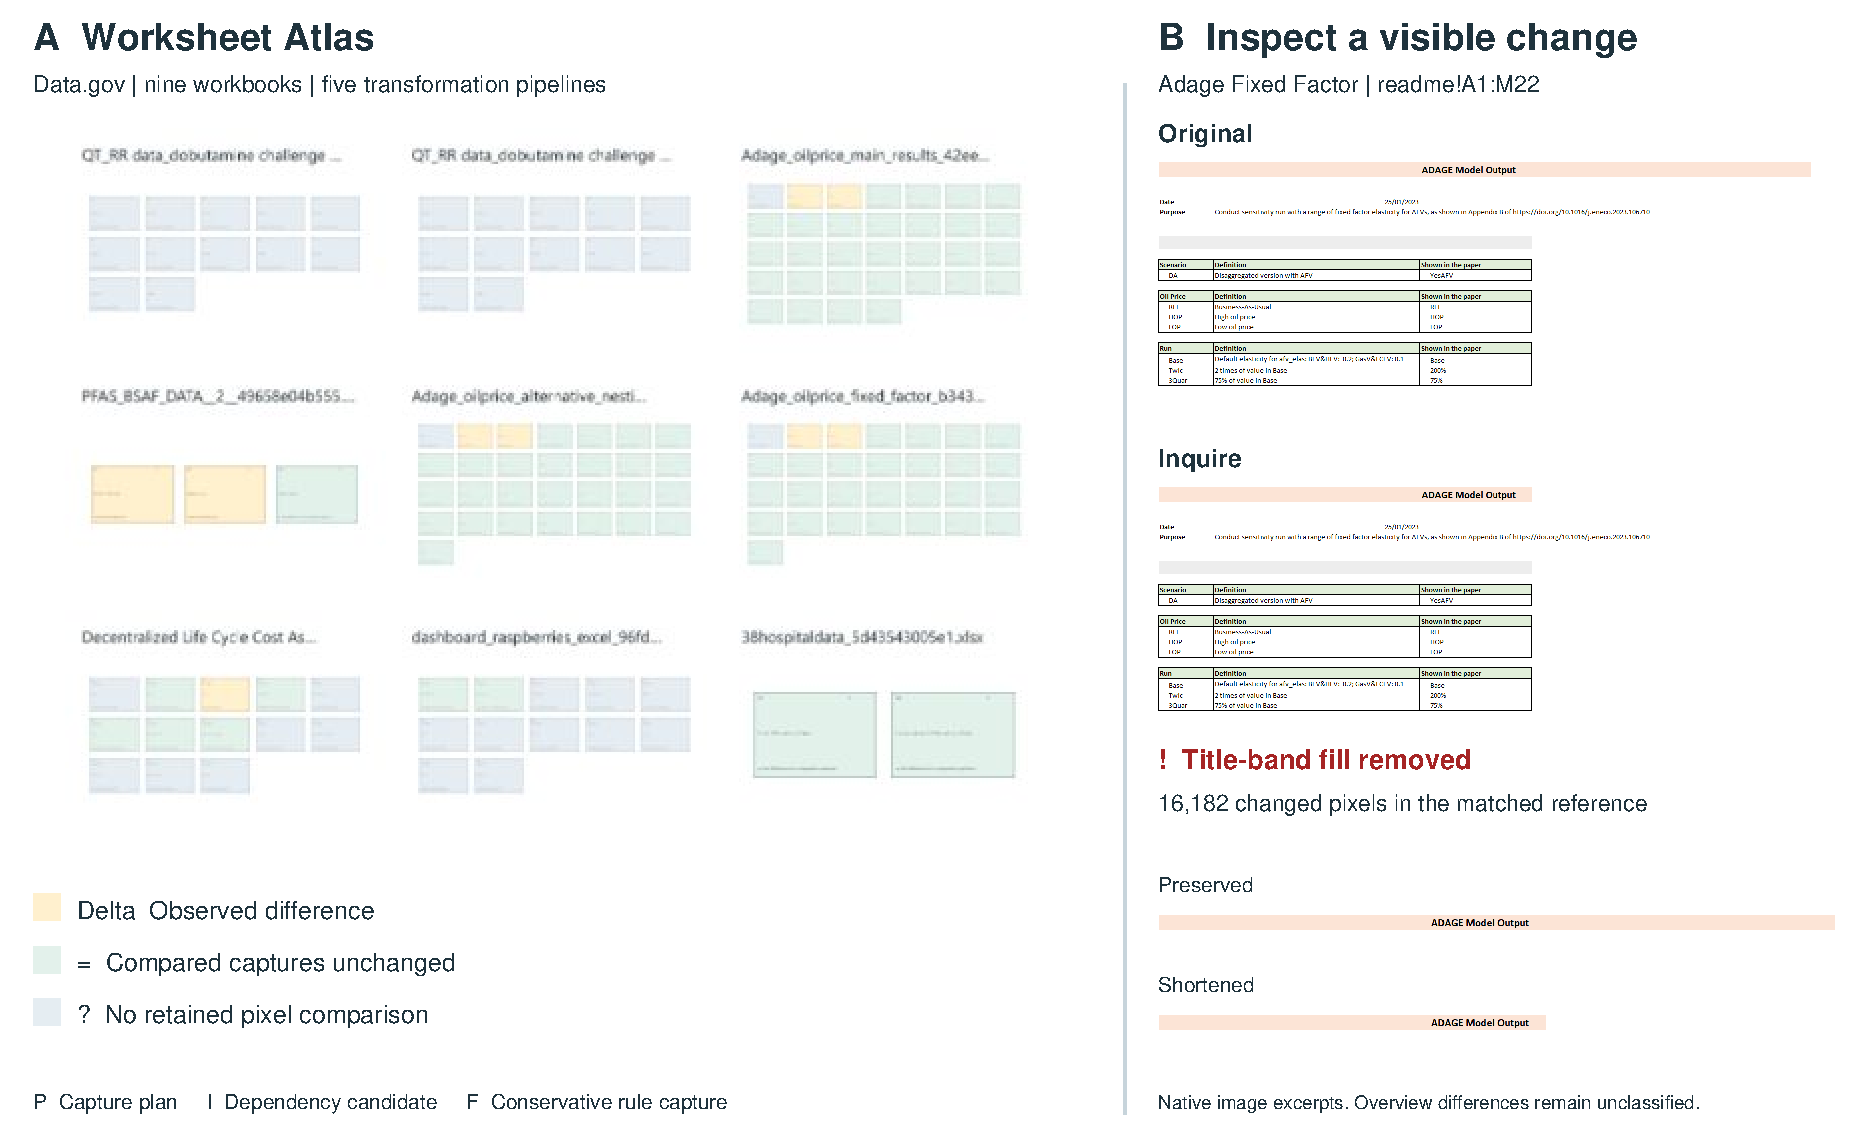
\includegraphics[width=.995\textwidth]{figures/atlas-cover.pdf}
\makeatletter
\def\@captype{figure}
\makeatother
\caption{From worksheet-level evidence to native image inspection. The left
view shows nine Data.gov workbooks and their 144 known sheets. Amber marks
recorded differences with unclassified cause, green denotes unchanged compared
captures, and blue-gray retains missing pixel coverage. Planning badges retain
recorded decisions independently of the outcome. The right view enlarges a
verified Adage title-band change in Inquire. The matched reference has 16,182
changed pixels. The displayed extent also remains shortened in Check Performance
and NXPowerLite, while SheetShrink and XLStylesTool preserve it. These grouped
observations concern this reference range.}
\label{fig:atlas-stage09}
\end{minipage}
\par\medskip

\noindent\begin{minipage}[t]{\textwidth}
\setlength{\multicolsep}{0pt}
\begin{multicols}{2}
\begin{abstract}
Checking whether a spreadsheet transformation changes its appearance can
require rendering large worksheets in Excel. DeltaSieve uses differences in
worksheet XML to select regions for native image comparison. It resolves cell
values, inherited formatting, row and column geometry, and dependencies of
conditional formatting and charts. Unresolved dependencies trigger broader
captures. The selected regions are rendered in Excel and compared pixel by
pixel. Separate opening, saving, and rebuilding controls record changes
introduced by Excel during preparation. The comparison study is organized
around 49 workbooks from Data.gov, Destatis, and Enron and five transformations
produced by SheetShrink, NXPowerLite, XLStylesTool, Check Performance, and
Inquire. Controlled examples show how removing a cell fill or an inherited
border changes the rendered worksheet. Reports connect findings to worksheet
coordinates, paired images, capture geometry, and execution measurements.
\end{abstract}
\end{multicols}
\end{minipage}}
\maketitle

\section{Introduction}
The introduction is being developed from the primary-source design study and the measured behavior of the implementation. This initial project verifies the manuscript build before the complete research-based draft is written.
\section{Preservation and Comparison Contract}
% Working prose derived from the paired-rebuild validation contract.
\subsection{Inputs, states, and observations}
DeltaSieve validates a pair of spreadsheet states produced by a transformation.
The package representation supplies evidence about where visible changes could
occur. Native Excel rendering supplies the image observations for selected
regions. A candidate is a
reason to inspect a region; pixel inequality is an observation that still needs
attribution.

The fast comparison uses Original and transformed workbooks after a full rebuild
and save in their existing, separately owned Excel processes. This gives both
partners the native recalculation step. Stored and ordinary-saved XML controls
remain available for follow-up. Their changes explain potential causes without
automatically enlarging the rebuilt-pair capture plan. An independently requested
Check Performance comparison has its own transformed state and coverage.

\subsection{Relevant visual area and candidate coverage}
The relevant area includes values, formulas, effective visible formatting, text
overflow, and objects. A union across relevant input states is needed to cover
content removed by a transformation. Empty trailing geometry has a separate
contract. The capture plan must retain enough evidence to distinguish a change
inside the relevant area from a larger or smaller exterior canvas.

Candidate selection considers changed cell properties and layout, as well as
regions affected through conditional formatting and graphical dependencies.
Style and shared-string references require comparison of their effective
contents because saving can renumber the corresponding tables. Supported
reference reasoning can exclude a dependent region when its rule and inputs are
unchanged. A changed dependency makes its affected region a candidate. Unresolved
reference semantics require explicit fallback coverage.

A selected-region comparison does not by itself demonstrate that every relevant
change in the workbook was selected. We evaluate that property using independently
rendered reference areas and controlled mutations. The evaluation must record
which reference cases completed and which exceeded their budgets.

\subsection{Verdicts, failures, and reusable evidence}
A successful comparison requires usable evidence from both partners. Missing
hashes, failed native commands, and timeouts remain unsuccessful outcomes.

The raw pixel and geometry observations remain attached to a finding after
review. Product regressions, rendering variation, environment-dependent values,
and verified capture-extent differences have separate classifications. A volatile
formula path explains a possible cell-value change while other changed pixels
in the same image can require further analysis. No global pixel tolerance is
assumed.

Reusable observations bind the input states, relevant configuration, producing
validation implementation, and declared rendering environment. Package-content
identity is evaluated independently of ZIP entry order and compression. Reusing
a completed study preserves its source manifest and compatibility checks.
Portable reports retain the observations and their provenance for inspection
without rerunning Excel.
\section{Method}
\begin{figure}[!ht]
\centering
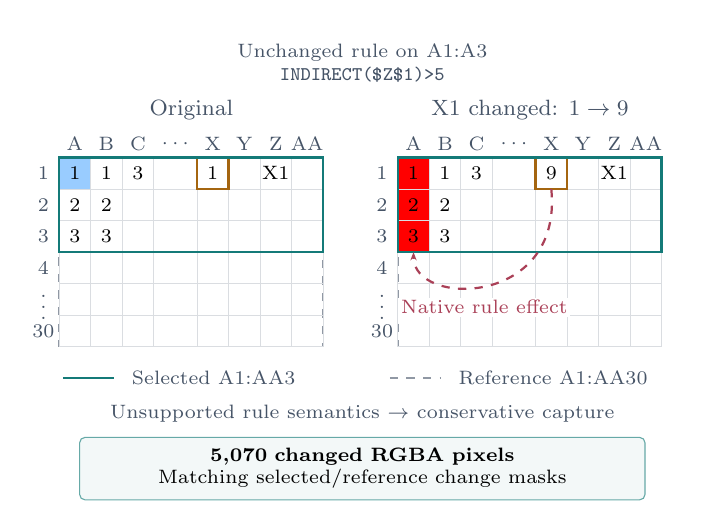
\begin{tikzpicture}[x=1cm,y=1cm,
  label/.style={font=\scriptsize,text=stateSlate,align=center},
  value/.style={font=\scriptsize,inner sep=0pt},
  selected/.style={draw=stateTeal,line width=.9pt},
  reference/.style={draw=stateSlate!60,dashed,line width=.65pt},
  effect/.style={-{Stealth[length=3pt]},draw=stateRose,line width=.8pt,dashed}]
\path[use as bounding box] (-.1,1.85) rectangle (8.35,-4.15);
\definecolor{nativeBlue}{HTML}{99CCFF}
\definecolor{nativeRed}{HTML}{FF0000}
\definecolor{editedCell}{HTML}{A46510}
\node[label] at (4.15,1.4)
  {Unchanged rule on A1:A3\\\texttt{INDIRECT(\$Z\$1)>5}};

% Both panels use the same address layout. The omitted columns and empty rows
% make room for legible values while preserving the tested range endpoints.
\foreach \offset/\title/\changed/\input in {0/Original/0/1,4.3/{X1 changed: $1\rightarrow9$}/1/9} {
  \begin{scope}[xshift=\offset cm]
  \node[label,font=\footnotesize] at (1.98,.8) {\title};
  \draw[reference] (.3,.2) rectangle (3.65,-2.2);
  \ifnum\changed=1
    \fill[nativeRed] (.3,.2) rectangle (.7,-1);
  \else
    \fill[nativeBlue] (.3,.2) rectangle (.7,-.2);
  \fi
  \foreach \xx in {.3,.7,1.1,1.5,2.05,2.45,2.85,3.25,3.65} {
    \draw[stateSlate!20,line width=.3pt] (\xx,.2) -- (\xx,-2.2);
  }
  \foreach \yy in {.2,-.2,-.6,-1,-1.4,-1.8,-2.2} {
    \draw[stateSlate!20,line width=.3pt] (.3,\yy) -- (3.65,\yy);
  }
  \foreach \xx/\column in {.5/A,.9/B,1.3/C,1.775/{$\cdots$},2.25/X,2.65/Y,3.05/Z,3.45/AA} {
    \node[label] at (\xx,.37) {\column};
  }
  \foreach \yy/\row in {0/1,-.4/2,-.8/3,-1.2/4,-1.6/{$\vdots$},-2/30} {
    \node[label] at (.1,\yy) {\row};
  }
  \foreach \xx/\yy/\number in {.5/0/1,.9/0/1,1.3/0/3,.5/-.4/2,.9/-.4/2,.5/-.8/3,.9/-.8/3} {
    \node[value] at (\xx,\yy) {\number};
  }
  \node[value] at (2.25,0) {\input};
  \node[value] at (3.05,0) {X1};
  \draw[editedCell,line width=.9pt] (2.05,.2) rectangle (2.45,-.2);
  \draw[selected] (.3,.2) rectangle (3.65,-1);
  \end{scope}
}

% This arrow depicts the observed native effect. The tested selector records
% unsupported rule semantics and captures conservatively rather than resolving it.
\draw[effect] (6.55,-.2) .. controls (6.7,-1.7) and (4.8,-1.7) .. (4.8,-1);
\node[label,text=stateRose,fill=white,inner sep=1pt] at (5.7,-1.7)
  {Native rule effect};
\draw[selected] (.35,-2.6) -- (1,-2.6);
\node[label,anchor=west] at (1.1,-2.6) {Selected A1:AA3};
\draw[reference] (4.5,-2.6) -- (5.15,-2.6);
\node[label,anchor=west] at (5.25,-2.6) {Reference A1:AA30};
\node[label] at (4.15,-3.05)
  {Unsupported rule semantics $\rightarrow$ conservative capture};
\node[draw=stateTeal!65,fill=stateTeal!5,rounded corners=2pt,
  text width=6.9cm,align=center,font=\scriptsize,inner sep=4pt] at (4.15,-3.75)
  {\textbf{5,070 changed RGBA pixels}\\Matching selected/reference change masks};
\end{tikzpicture}
\caption{Schematic reconstruction of a native-tested synthetic control~\cite{indirectcontrols}.
X1 changes from 1 to 9 while Z1 retains ``X1'' and the conditional rule remains
unchanged. The rule turns A1:A3 red. The tested selector uses conservative capture
of A1:AA3 because the rule is unsupported. Its change mask matches the independent
A1:AA30 reference. Intermediate
columns and empty rows are compressed.}
\label{fig:validation-overview}
\end{figure}

\subsection{Observe an explicit state pair}
The fast production strategy opens original and transformed workbooks in separate
owned Excel processes and rebuilds them in place. A configured worker pool may
lease existing processes across file pairs. Measurements must distinguish
per-workbook opening from process and add-in initialization, and record the
reuse policy when reporting campaign throughput. It compares their rebuilt
states. Saved-input and pre-rebuild controls can explain changes introduced by
Excel's own save or calculation behavior. Enabling additional controls incurs
separate cost and must be recorded in the run configuration. A cached control
is reusable only under its source and environment compatibility requirements.

Legacy XLS conversion precedes the XLSX comparison subject. A workbook requiring
repair, inaccessible protected content or an unsuccessful save receives its own
outcome. Missing evidence cannot yield equality. A host process existing in the
operating system and an Office.js add-in responding are separate liveness signals.
Neither proves that calculation or capture work has advanced.

\subsection{Select potentially affected regions}
The XML analysis compares cell values and formulas together with their effective
style context. A style index is local to a package. The same index can identify
changed properties, while different indices can identify equivalent properties.
The planner resolves that context before interpreting cell differences.

Layout analysis includes row, column and default-format effects. Stored row-height
attributes alone do not establish native effective heights. The native stage
therefore measures the relevant geometry. Content bounds include values,
formulas, visible fills and borders, and supported object extents. The union of
both states is important when an operation removes content.

Conditional-formatting analysis follows supported references. When a referenced
input changes, its dependent application region becomes a candidate regardless
of whether a particular rule outcome might remain the same. Unchanged supported
rules and inputs can exclude a region. Unknown formulas, namespaces or extensions
retain the documented fallback. Chart selection similarly considers supported
formulas, referenced inputs and caches, with conservative handling of unresolved
cases. The rule inventory and its unsupported cases are versioned with the tool.

\subsection{Measure and render}
Candidate regions are clipped to the justified content envelope. Connected regions
are subdivided according to native measured image size. A fixed row count cannot
predict the visible size of hidden or irregular rows. Zero-area regions have an
explicit non-rendered outcome. Geometry and image batches have separate controls,
allowing measurement overhead and rendering memory to be tuned independently.

Office.js image results become available after synchronization. Hash calculation
therefore follows synchronization of the requested image batch. Compatible equal
hashes can avoid transmitting and retaining equal images under the recorded
transport policy. Actual unequal images remain evidence. Hash transport, image
retention and scientific coverage are separate choices.

\subsection{Bounded execution and recovery}
Resident workers receive commands over session-scoped WebSockets, while image
uploads use bounded HTTP requests~\cite{deltasieveexecution}. Durable commands,
image receipts and results remain authoritative across reconnections. Duplicate
delivery must preserve an in-progress command and acknowledge an identical
completed result without running it again. Capture and upload overlap within
bounded tile, pixel and encoded-memory windows. Office calls remain serial
within an individual workbook.

Each comparison group owns its Excel processes and an isolated WebView profile.
Cleanup records requested termination separately from confirmed exit. A retained
clean-desktop control reproduced a peer taskpane restart under shared-profile
cleanup; per-group isolation passed the corresponding two-group control and a
four-group sequence. This observation motivates resource ownership in the tested
environment. It does not establish that every startup delay is caused by stale
profiles or registrations.

\subsection{Retain outcomes and explain uncertainty}
The report records selected regions, compared states, configuration, timings and
failures. Pixel diagnostics provide changed-pixel counts, channel deltas and
magnified regions. They do not assign a regression verdict on their own. Formula
dependency traces can identify a supported path to a volatile function without
explaining every changed pixel in the surrounding image.

Portable reports retain images using relative paths and integrity manifests.
Their static viewer needs no Excel installation or running control API. Run
metadata must be reviewed for local paths and publication-sensitive content
before public release. Historical replay requires recorded event history and
cannot reconstruct observations that were never retained.

\section{Evaluation}
RQ1 asks whether the selector captures the known visible effects in the tested
mutation classes and independent reference sample. RQ2 measures how much native
capture work and elapsed time it avoids. RQ3 examines the reproducibility and
investigability of retained findings, including failures and rendering variation.

\subsection{Corpus identity and outcome accounting}
The evaluation treats Data.gov, Destatis and Enron as distinct populations.
Archive checksums, member names and duplicate occurrences identify each selected
corpus version. Legacy XLS conversion is reported separately from XLSX cleanup.
The ongoing Enron fallback selection contains 20,872 inputs, of which 20,503 have
prepared artifacts and 369 have unsuccessful preparation outcomes. Its visual
scope contains 16,799 workbooks. These are preparation counts for the current
selection, not final visual-validation results.

A dated evaluation cutoff will report compared workbooks, differences, failures,
unsupported representations and unfinished work. Repeated attempts have their own
counts. An unchanged package can bypass visual work under an exact input-identity
check, but a failed capture cannot contribute an equality observation. The full
recursive Enron XML-derived corpus is a separately identified population.

\subsection{Sampling and reference controls}
The random evaluation sample is selected from a frozen eligible frame with a
recorded seed before inspecting visual findings. Strata use corpus identity,
package size and structural features available before validation. Low-reduction
and unchanged files remain represented. A separately labelled development stress
set contains large and historically problematic workbooks.

Feasible sampled files receive full native reference captures over the relevant
visual area using a capture plan independent of the candidate selector. A
full-reference timeout remains in the denominator. It is not replaced silently
by an easier workbook. Mutations with known visible effects cover cell values,
styles, geometry, conditional dependencies and objects. Mutations that Excel
normalizes away are reported separately.

\subsection{Detection and cost metrics}
A selector miss is a native reference difference outside the selected coverage.
Report detection by mutation class and by completed reference workbook. A changed
capture is counted separately from a confirmed transformation regression.
Unsupported references, failed geometry reads and missing partner images retain
explicit coverage outcomes.

Cost measurements separate XML planning, geometry, native rendering, transfer,
image comparison and persistence where instrumentation permits. Report image
count, compared pixels and retained bytes alongside elapsed time. Batch and
concurrency experiments use matched inputs and repeated runs. A changing
production queue does not identify the causal benefit of a tuning parameter.
Full-corpus cost estimates use measured visible geometry and stratified samples,
with uncertainty and assumptions about hidden regions and object extents.

\subsection{Current verification boundary}
The portable-viewer smoke experiment retained a deliberately different pair,
loaded its images through relative static assets and displayed its diagnostics
without a running control API. An empty-partition test verified explicit selected
and excluded counts without opening Excel. These tests verify execution and
reporting boundaries. They do not establish selector recall.

\textit{Evaluation freeze pending.} Complete the independent mutation matrix,
seeded native reference sample and matched cost tables before making detection
or speedup claims. Retain unresolved development cases and the original pixel
observations when a later retry or software fix changes their classification.

\section{Related Work}
\subsection{Spreadsheet dependencies and testing}
Spreadsheet slicing connects dependency analysis with integrated testing and
fault localization~\cite{slicing}. DeltaSieve uses supported dependencies to
select native observation regions. The two methods have different adequacy
obligations. Formula-dependency coverage alone does not cover every visual effect.

\subsection{Workbook comparison and native evidence}
Spreadsheet Compare documents workbook comparison reports with formula and
cell-format categories, including hidden sheets~\cite{spreadsheetcompare}.
This is an important existing capability. DeltaSieve's comparison must examine
native rendered effects, candidate selection and corpus execution explicitly,
using common test inputs where the installed tools support them.

\subsection{Cross-system testing and parsing}
SQuaLity examines barriers to reusing database test suites across systems,
including configuration and execution dependencies~\cite{squality}. This suggests
recording the renderer and environment when reusing observations. The analogy
does not transfer database test adequacy guarantees to spreadsheet rendering.
SheetReader's specialized parsing work~\cite{sheetreader} is relevant to efficient
package inspection, whose cost must be separated from native rendering cost.
Further work will examine change-impact analysis and visual regression testing
with verified primary sources.

\section{Discussion and Limitations}
The central risk is an incomplete candidate model. A proof for supported inputs
must state its dependencies and applicable namespace or rule subset. Unknown
features need a capture fallback or an explicitly incomplete outcome. Runtime
limits and failures reduce achieved coverage and must remain in the report.

A native renderer is also an experimental dependency. Recalculation, volatile
formulas, file-location functions and rendering variability can change output
without a transformation defect. A volatile dependency trace explains a supported
path rather than every image difference. A white exterior canvas difference
requires geometry and containment checks before classification. No global pixel
tolerance is inferred from one rare anti-aliasing case.

The Observatory reduces the effort of investigating these outcomes. Portable
reports and a future recorded-event replay can demonstrate execution and make
findings inspectable. They do not establish authenticity solely by being detailed,
and replay cannot supply missing historical telemetry. Scientific claims rely on
source identities, implementation versions and the independent evaluation.

\section{Conclusion}
DeltaSieve combines dependency-aware region selection with native rendering
and inspectable evidence. The bounded experiments demonstrate concrete
findings and fallbacks. Corpus-wide recall and matched capture cost remain
open.

\label{sec:main-text-end}
\section*{Acknowledgment of AI Assistance}
OpenAI ChatGPT and Codex assisted with drafting and editing the Abstract and
Sections I--VII, literature discovery and organization, implementation and
refactoring, test and experiment scripts, figure-generation code, and analysis
of retained experiment evidence. This assistance included the method diagrams,
XML examples and execution visualizations. Local agent workflows using these
systems also supported overnight validation campaigns by inspecting status and
logs, investigating stalled attempts, and documenting candidate visual
regressions for author review.

The author directed development, reviewed source code, and performed manual
testing and debugging. Agent observations supported investigation. Reported
validation outcomes are grounded in the retained native captures and comparison
records. The author remains responsible for the scientific claims, references,
evidence selection, originality and final submitted content.

\bibliographystyle{IEEEtran}
\bibliography{references}
\end{document}
